\documentclass[11pt]{article}
\usepackage{geometry}                % See geometry.pdf to learn the layout options. There are lots.
\geometry{letterpaper}                   % ... or a4paper or a5paper or ... 
%\geometry{landscape}                % Activate for for rotated page geometry
%\usepackage[parfill]{parskip}    % Activate to begin paragraphs with an empty line rather than an indent
\usepackage{graphicx}
\usepackage{amssymb}
\usepackage{epstopdf}
\usepackage{indentfirst}
\DeclareGraphicsRule{.tif}{png}{.png}{`convert #1 `dirname #1`/`basename #1 .tif`.png}

\title{Small Screen, Big Strategy: Bringing Real-Time Strategy to Mobile Devices}
\author{Edward Bramanti}

\begin{document}
\maketitle
\abstract{A proposed interface design for how to bring real-time strategy to the mobile gaming scene. I will argue that the biggest challenge to real-time strategy on mobile is a combination of overwrought interface design and poor controls. With a simplified and clean interface combined with intuitive, easy-to-remember controls, it will provide the best possible mobile RTS experience for users.}
\pagebreak
\section{Introduction}
In the past few years, mobile operating systems have become a hub for both independent developers and game studios alike to publish video games that their consumers can hold in the palm of their hand. Mobile game development once used to be a frontier; now, it seems as though a new game comes out every few weeks, and they battle for the addiction of their consumers. While many different genres of mobile games have been produced, from tower defense to adventure to even massively multiplayer, real-time strategy remains a genre mostly untouched by mobile game developers. One's initial reaction may be to believe that lack of interest in real-time strategy (or RTS) games is responsible for few games being published in that genre. Nevertheless, as this design will outline, a lack of intuitive controls and user interface has prevented the genre from thriving on mobile. Many developers have been met with interface design challenges. One example of this is a result of lacking hardware devices outside of the touchscreen (such as a mouse and keyboard, or even a controller with buttons). My user design will show how mobile strategy is the future of challenging, yet rewarding mobile gaming. Empowering the users by utilizing every inch of screen is the key foundation to building a successful mobile RTS interface.
\section{Design \& Layout}
To successfully approach designing a user interface for mobile RTS, my approach will be to play to a touchscreen's strengths, and conform to design principles in mobile operating systems.
	\subsection{Unit Selection}
	To select a unit within the proposed design, a user will use just a finger and tap on whatever unit they want to control. While this is simple enough, the challenge arises when a user wants to select multiple units, because of a lack of draggable input using a mouse cursor. I decided to take an approach similar to Halo Wars. Halo Wars employs a reticle, and when a user holds down the A button on the Xbox 360 controller, an overlay appears that shows units in the selection circle. Since the user's controller is the touchscreen itself, the same action will occur when one holds down their finger on the screen. After a small delay, the selection circle will expand from the held touch input, and allow multiple units to be selected at once.
	\begin{figure}[h]
	\begin{center}
	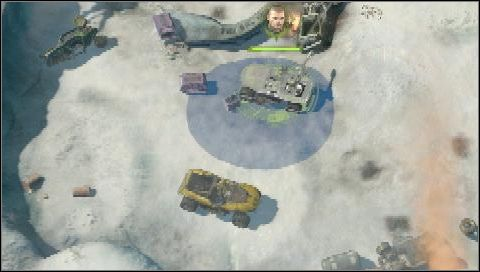
\includegraphics[height = 2.5in]{blue-selection}
	\caption{How unit selection is implemented in Halo Wars. When a user holds down the A button, a ring appears that allows multiple units to be selected. The implementation is similar here, but with your finger instead!}
	\end{center}
	\end{figure} \\
	\indent When a unit is selected, stats will be displayed about them centered at the bottom of the screen. If multiple units are selected, they will be displayed in groups by type in the top-left corner of the screen. This will allow a user to both view attributes below their selection, and view their selected units in a status bar at the top of the screen (which, in mobile OSes, is always located at the top of the touchscreen.)
	\subsection{Minimap}
	One of the most important information displays to anyone playing a real-time strategy game is the minimap. The minimap is incredibly useful to see where units are located, and where friendly units are deployed. It allows for users to navigate the map quickly; by selecting a location on the map, it allows the camera to snap quickly to that location on the game map. The minimap also provides the user with a way to see where enemies are attacking, and ``pings'' information to the user when enemy attacks occur.\\
	\indent The biggest challenge of implementing this on a mobile device, as opposed to a computer, is the size of the smartphone screen. I believe that the minimap is essential for the user interface in the RTS genre, but I also believe that cluttering the camera view of the map with too many tooltips will make it difficult for the user to quickly issue commands to their units. Therefore, I propose a two-size minimap.
	%	Picture will go here of the minimap.
	\begin{figure}[h]
	\begin{center}
	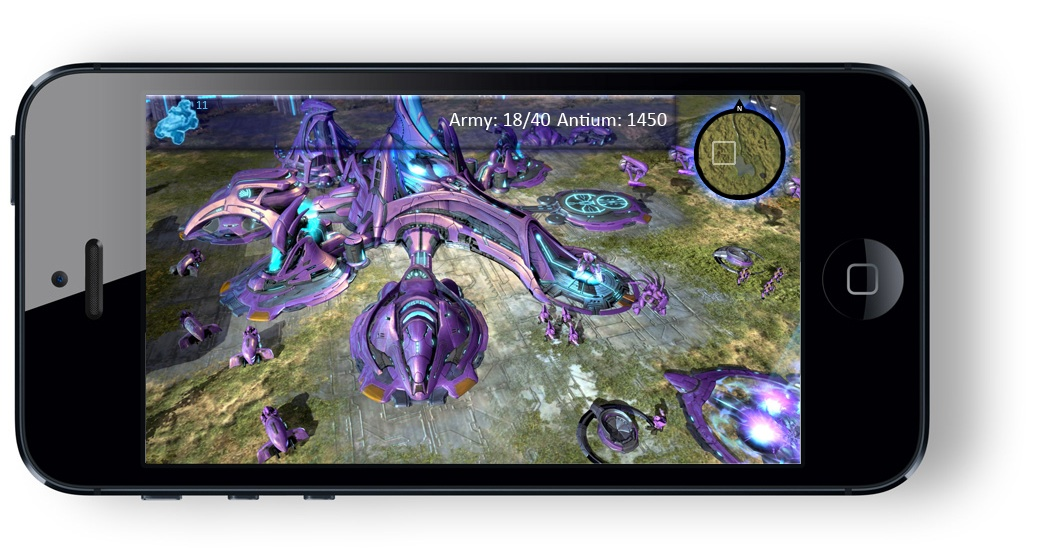
\includegraphics[height = 2.5in]{minimap}
	\caption{An example of a mock-up minimap design is shown in the top-left corner. Users will interact with the minimap heavily in real-time strategy, which is why placement is key.}
	\end{center}
	\end{figure} \\
	\indent In a normal view, the user will have a very small glimpse of the minimap, as pictured above. It will show their current camera view on the minimap, and a very small representation of unit locations and map. To conquer the issue of screen space, a tap gesture will be employed on the minimap. When a user taps the minimap once, it will cause the minimap to go full screen. This minimap will allow the user to see a bigger, ``computer-sized'' minimap as opposed to providing a static, small minimap that is close to useless anyways. This will allow a user to see everything going on, and their current camera location behind the overlay. To exit the enlarged minimap, the user will have two options. They can either close the enlarged minimap by selecting outside of the overlay to dismiss. The other option would be to select an area of the map where they would like the camera to snap to. This will allow for the snap-to-location camera functionality that PC RTS gamers have, while scaling the experience to work within the confines of screen space and touchscreen input.
	\subsection{Unit Movement}
	Now that unit selection and the minimap interface has been explained, unit movement is based off of many of the same principles. After successfully selecting units on the map, you can use either the minimap overlay or within your camera view to move your units. With a tap using either of those methods, your units will be able to move. This will allow unit movement to be simple and easy to remember. After a tap, while units are moving, holding a tap in a different location will allow a user to chain movement commands together, much like Shift + Right Click in Starcraft II.\\
	\begin{figure}[h]
	\begin{center}
	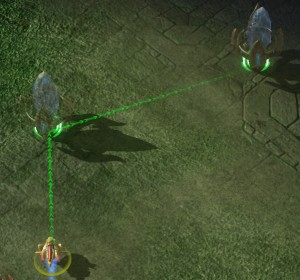
\includegraphics[height = 2.5in]{sc2-movement-queue}
	\caption{An example of queued movement in Starcraft II. Shift + Right Click allows for units to chain together movement, and draws a path to the next movement point.}
	\end{center}
	\end{figure} \\
	\indent To attack either a group of units or a base, a double tap on the enemy object will cause an attack command to be issued. In addition, double-tapping on an area in the minimap view will issue the attack-move command, meaning that if any enemies are encountered along that path, the user's units will attack. This is, in some ways, an extra option; developers will already have their units attack automatically when enemies are within a certain range, but it is definitely useful to the hardcore real-time strategy community. In addition, if an attack-move command is issued and users hold-tap to queue, it will queue up attack move commands.
	\subsection{Camera Control}
	For camera control, I took inspiration from both iOS and Android Design paradigms. Pinching with two fingers outward will allow the user to zoom in on their current view, and conversely, inward would allow the user to zoom out. It seemed natural to use this in the control scheme so that users would not becomed confused when a two-finger pinch causes a different action to happen, such as a unit selection box. \\
	\indent In addition, camera rotation is essential for users playing a real-time strategy game. A user needs to be able to see from a different direction than just a fixed north; therefore, the user needs intutitive controls to dynamically adjust to the situation. Once again looking at universal gestures in the mobile OS, I took a page from Google Maps' two finger rotate to view at any angle. This will allow the user to adjust the camera's direction quickly and effectively.
	\subsection{Building Management \& Interface}
	\begin{figure}[h]
	\begin{center}
	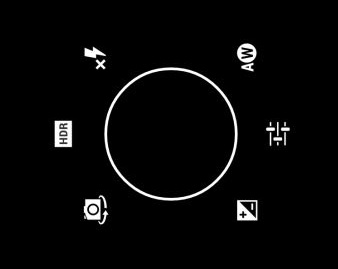
\includegraphics[height = 2.5in]{android-camera}
	\caption{An example of what a building interface will look like when a user selects a building. Pictured here is the Android Jellybean Camera interface, tilted 90 degrees to the left. An interface similar to this one will be overlayed on top of the selected building on unit tap.}
	\end{center}
	\end{figure}
	For building management, my goal was to make it easy for players to be able to queue up units and research while still maintaining a touchscreen design. In otherwards, I wanted users to be able to quickly see at a glance what's going on quickly with each of their different buildings. I found inspiration in the Stock Android Camera interface, where users hold their finger down and a fanned-out circle appears from their finger. This allows users to toggle different cameras, enable HDR, or even change white balance. Using a similar technique, instead of holding down their finger on a building, when a user taps a building a similar fan-like circle appears around it. \\
	\indent A good illustration of how this will look would be to imagine a barracks with three unit types: a soldier, an anti-infantry unit, and some other special unit. Each unit would be displayed on the right side of the fan, with a unit count next to the pictorial designation of what type of unit they are. Each little fan section, when soldiers are being queued to be built, will fill with a color as units are trained. On the left side of the fan is where upgrades will be applied to certain units. \\
	\indent This illustration above is an example of the adaptive interface that this fan will provide on a building. For my design, if a developer wants to create a building type, unit creation will be on the right according to my design guidelines, and research will always be on the left. The only exception to this rule will be if the building itself is for research only, or if it is some special type of building used for only resource collection, etc. The interface adapts to the many different ideas that developers have, while providing them guidelines on how to organize their building tasks.
\section{Usage Scenarios}
	\subsection{Creating a Real-Time Strategy Game for Mobile Devices}
	In its simplest form, this is the reason why this interface was designed: to create a simple and easily controllable interface for a developer to design a game within. According to critics, the difficulties that real-time strategy games have always faced outside of the traditional PC market is lacking a mouse and keyboard. My entire interface design is not only to prove these critics wrong, but also to show that the reason for a lacking RTS market outside of personal computers is because developers have implemented a poor user interface and control system for the user. \\
	\indent The type of real-time strategy that can be implemented using this interface design and layout is pretty endless. While many tower-defense RTS games have already found success on the market due to a time-lapse between tower creation, there are many other genres of real-time strategy that will benefit from this interface. In addition, this usage scenario need not apply to only one device; the interface is designed to be dynamic, regardless of screen size, buttons, etc. This is due to the universal importance of the touchscreen to smartphones; almost all modern smartphones have a touchscreen interface, which means using this interaction style will be seamless and simple for today's devices.
	\subsection{Companion App: RTS/FPS Hybrid between Console/PC and Mobile Devices}
	One unique way this design could be used would be a way to provide a companion app that would enhance the gameplay of a First-Person shooter while also providing a strategy element. This would allow both the mobile companion and the larger console game to be pushed to a much larger scale than ever before. For example, there could be 2 Battle Commanders on their mobile devices (pretty close to an Ender's Game scenario). They will be able to interact with the battlefield in a certain way, where they will have control where to move troops. When a confrontation between two squadrons arises, the console players will be pushed into the action to see who can come out on top. This will allow a way for consoles and mobile devices to be companions, and for a fun way to play while on the go. Even on the move, though, there is still a console experience as you control unit movements using commands from the interface.
\section{Design Rationale}
	\subsection{Unit Selection}
	\begin{figure}[h]
	\begin{center}
	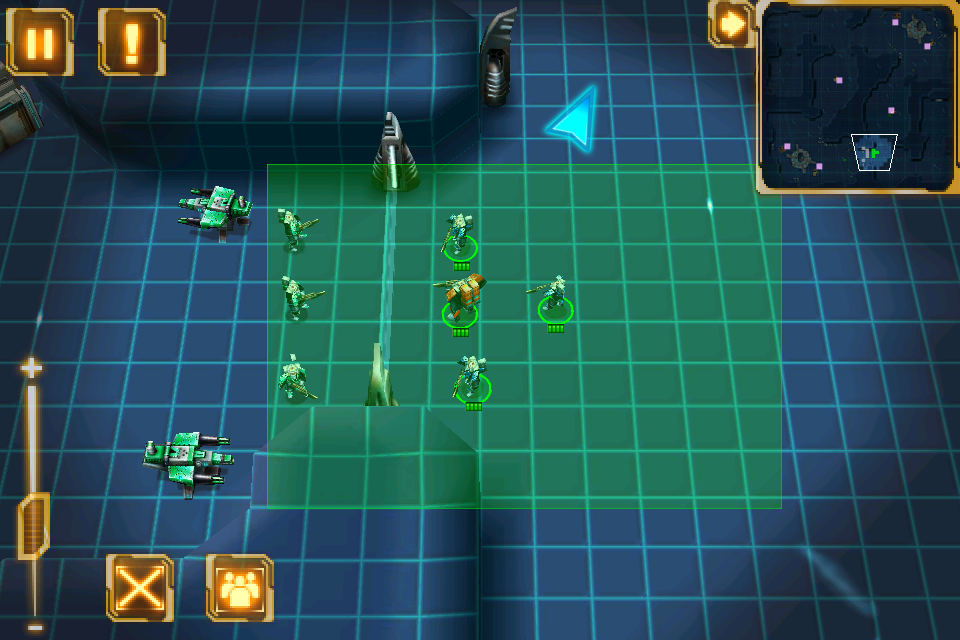
\includegraphics[height = 2.5in]{starfront-selection}
	\caption{An example of unit selection in a mobile RTS, ``Starfront: Collision.'' In this example, a user does a two-finger gesture, with each finger in diagonally opposite corners, to select units.}
	\end{center}
	\end{figure}
	There are a few mobile RTS games on the market today. One notable example is Starfront: Collision, which is available for iOS devices. Starfront's approach for selecting units, or multiple units, is to use a pinch, or two-finger touch, to select a group of units. The biggest problem with this approach is that it directly contradicts the design guidelines of mobile operating systems. While this conforms to the design guidelines of mouse selection on PC, it does not translate well to the mobile experience. This is why I decided to use a radial selection method: a user holds their finger on the screen, and it expands to encompass units over a certain area. It better conforms to the ideas of touch input, while in some cases lacking the direct manipulation users are used to when playing real-time strategy with a mouse and keyboard. Nevertheless, I believe this to be a stronger approach than two-finger select, as it interferes with the guidelines of a mobile OS and will confuse the user expecting the gesture to zoom-in the camera.
	\subsection{Minimap}
	The Minimap Interface was designed to overcome the inefficiency that is proven by Fitts' Law. Since the target of the minimap is too small, some mobile RTS's have attempted to overcome that by drawing a bigger minimap in the top-right corner of the screen. Nevertheless, an issue results from that approach: less room for the user to select objects on the screen, and even to issue movement commands. On top of that, minimap control suffers from the same Fitts' Law issue that was originally trying to be fixed. The selection area for moving the camera view around the map is small, which makes it difficult for accurate camera placement. This is why I chose to add an expandable map interface: it makes the minimap target huge, while at the same time preserving all the action happening on-screen. The advantage of this approach is that it is dynamic as well; in the heat of battle, the user will not have the minimap getting in the way. This will allow the user to be immersed in the action on-screen, while still being alerted (or ``pinged,'' in my interface design language) to other events happening on the smaller minimap.
	\subsection{Unit Movement}
	For unit movement, the goal setting out was to limit the amount of taps that the user would need to memorize, and provide feedback of what the user's commands were causing to occur. The hold-tap input made sense for chaining commands because it would both provide feedback to the user by drawing a next-movement line and preventing interference from user modification to movement patters. If a user can see visible navigation as to where their units are going, it can only enhance the experience. Keeping the tap commands simple will limit the errors a user will make; there is no specific halt command, but by using a quick move by tapping once, it will cause units to stop when they reach your last tap. This sequence design will help users to give complex commands, while making it easy to cancel if need be.
	\subsection{Camera Control}
	To rationalize my design for camera control, I will address two examples: one illustrating why Starfront: Collision's implementation makes camera control difficult for the user, and mobile OS user interface control for controlling the ``camera'' of common map applications on mobile operating systems. \\
	\indent In Starfront, users are provided with a slider on the left side of the interface (as seen in Figure 5), which allows for users to zoom in by sliding up, and zoom out by sliding down. Nevertheless, as mentioned in the Unit Selection rationale, it directly is in conflict with what the gesture does across the OS. A user will use the two-finger pinch gesture, and instead of zooming in, they will be met with a unit selection box. This app is an example of a failure in implementing direct manipulation that corresponds to what most of the mobile OS does in regards to that gesture.
	\begin{figure}[h]
	\begin{center}
	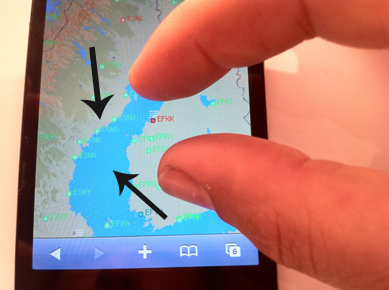
\includegraphics[height = 2.5in]{iphone-two-finger-pinch}
	\caption{An example of a two-finger pinch gesture common on many mobile operating systems.}
	\end{center}
	\end{figure} \\
	\indent A known paradigm in mobile operating systems is the two-finger pinch gesture; for example, in mobile map applications, two-finger pinch will zoom in and zoom out, respectively. Two-finger radial movement will cause the direction of the map to change. In my implementation of an RTS interface, I want to match this paradigm. This is a small way to reduce the user's cognitive load, and have the commands they are issuing make sense. If other applications in the operating system utilize these guidelines, then this interface should be no different.
	\subsection{Building Management \& Interface}
	For mobile devices, I believe that cluterring up the already limited screen space will only make the user more error-prone as they execute actions. I believe that utilizing my building management interface will limit that error-prone behavior, while providing context to their current action. When a user selects a building, the commands fan-out around the building in a pie-menu fashion, showing the user their selection while displaying actions around it. This provides context to the user in the form of direct manipulation: the user wants to build something, so as they tap a building command options naturally form out of that tap. It provides the distinctive and clear set-up of a menu mental model as well: distinctive and clear choices always are mapped from left to right (research = left, units = right). 
\section{Usability Analysis}
	\subsection{Learnability}
	I believe that time for learnability will be easy utilizing this interface design, and the time it would take to learn would be low. This mobile RTS interface follows navigation guidelines of ``standardizing task sequences'', such as pinch-to-zoom and two-finger rotation for camera control. In addition, there are no more than two tap commands to memorize. Using commands that are similar to how the mobile OS itself is implemented can only increase learnability, as users perform these tasks across the operating system on a day-to-day basis.
	\subsection{Efficiency}
	Efficiency will be another strong point of this user interface. The goal of the interface was to simplify the amount of actions that would be needed to get units to move/interact/etc. to no more than two touches. This means that it takes less time digging through menus and searching for an option. In addition, the building fan interface will make all options available to the user at once, with categorization design guidelines. This can only improve efficiency as they approach memorizing what side represents what.
	\subsection{Rate of Errors}
	There is a chance for errors in the interface in a few spots. Looking specifically at the tap gestures, depending on developer implementation there could be rogue touch input that causes units to move where the user does not want them to. A rogue touch could also have the potential to cancel unit movement altogether, which means that their troops will have not responded as the user is under attack. In addition, while designed with smaller screens in mind, a smaller screen means less room to move units on the map and more of a chance to mistap. Since the size of the target location is significantly smaller, Fitts' Law will come into play. Even though the distance will be shorter because of the screen, the tap space will be much smaller which could cause a misregistration of the input, and possibly make it harder for the user to interact.
	\subsection{Memorability}
	Memorability will always be a difficult area, and not just because of a user interface. Real-time strategy games demand a mastery of a control scheme, map layout, and the core gameplay strategy to win. This is what has made this genre of game competitive even before the computer (chess is one notable example). Nevertheless, since I believe that simplifying the interface and standardizing task interfaces will cut down on the time it takes to memorize commands. If users already know how to use their mobile devices with a standardized set of guidelines that most developers conform to, this will as well. That's why I believe that even though memorability will be difficult due to the complexity of some real-time strategy games, my interface will allow the time to at least be reduced in memorizing movements and commands.
	\subsection{Satisfaction}
	Subjective satisfaction will be hard to measure without running an actual test, but I believe that this implementation will satisfy users. Users crave for a simplicity of interface, one that gets out of the way but also provides the power they need to complete tasks. My goal was to make the interface more dynamic than static, which allows many elements that normally take up screen space to get out of the way. Users will be able to focus more on playing the game than being shot down by an overwrought static interface.
\end{document}  